\subsection{Foundations}

\subsubsection{Notation}
We can define the following notation for probability:
\begin{itemize}
    \item We denoted the \textit{state space} or \textit{universal set} as $\Omega$ or $S$.
    \item An \textit{event} is a ``nice" subset of the state space, i.e. an event $A$ fulfils $A\subseteq\Omega$. The set of all events is often denoted by $\mathcal{A},\ \mathcal{E},$ or $\mathcal{F}$.
    \item A \textit{probability measure} $\prob$ is a map taking events as argument with
    \begin{itemize}
        \item $\prob:\ \mathcal{A}\to[0,1]$
        \item $\prob(\Omega)=1$
        \item For a countable index set $I$ with $(A_i)_{i\in I}$ being disjoint events, we have $\prob\brround{\bigsqcup\limits_{i\in I}A_i}=\sum\limits_{i\in I}\prob(A_i)$
    \end{itemize}
\end{itemize}
Set notations:
\begin{itemize}
    \item Intersection: $A\cap B=\brcurly{\omega\in\Omega:\ \omega\in A\text{ and }\omega\in B}$\\
    \begin{venndiagram2sets}[labelA={}, labelB={}, labelOnlyA={$A$}, labelOnlyB={$B$}, labelAB={}]
        \fillACapB
    \end{venndiagram2sets}
    \item Union: $A\cup B=\brcurly{\omega\in\Omega:\ \omega\in A\text{ or }\omega\in B}$\\
    \begin{venndiagram2sets}[labelA={}, labelB={}, labelOnlyA={$A$}, labelOnlyB={$B$}, labelAB={}]
        \fillA \fillB
    \end{venndiagram2sets}
    \item Complement: $A^c=\brcurly{\omega\in\Omega:\ \omega\notin A}$\\
    \begin{venndiagram2sets}[labelA={}, labelB={}, labelOnlyA={$A$}, labelOnlyB={$B$}, labelAB={}]
        \fillNotA
    \end{venndiagram2sets}
    \item Difference: $A\setminus B=\brcurly{\omega\in A:\ \omega\notin B}$\\
    \begin{venndiagram2sets}[labelA={}, labelB={}, labelOnlyA={$A$}, labelOnlyB={$B$}, labelAB={}]
        \fillANotB
    \end{venndiagram2sets}
\end{itemize}
We use the square cups $\sqcup$ to denote the disjoint union of sets. This means that $A_1\sqcup A_2$ implies that the two sets have no overlap and they are disjoint: $A_1\cap A_2=\emptyset$.\\
Discrete Uniform Distribution:\\
We require that $\Omega$ is non empty and finite. If every event $\omega$ is equally likely, we have a discrete uniform distribution. This means that
\[\prob(\{\omega\})=\frac{1}{|\Omega|}\ \forall\omega\in\Omega\]
Then the probability of an event $A$ is
\[\prob(A)=\frac{|A|}{|\Omega|}\]
We call this setting a discrete uniform distribution or uniformly random.\\
Ex: For a die, we have $\Omega=\{1,2,3,4,5,6\}$ and $\prob(\{\omega\})=\frac{1}{6}$.\\
Ex2: For two die we have $\Omega=\brcurly{(1,1),(1,2),\ldots,(6,5),(6,6)}$ and the probability of rolling a 1, 2, or 3 is
\begin{align*}
    &\prob\brround{\brcurly{1,2,3}}=\prob\brround{\{1\}\sqcup\{2\}\sqcup\{3\}}=\prob(\{1\})+\prob(\{2\})+\prob(\{3\})=\frac{1}{6}+\frac{1}{6}+\frac{1}{6}=\frac{1}{2}
\end{align*}
Some useful properties of probability:\\
For disjoint events $A,\ B$ we have $\prob(A\sqcup B)=\prob(A)+\prob(B)$.\\
Let $A,\ B$ be events with $A\subset B$. Then $\prob(A)\leq\prob(B)$
\begin{proof}
Define $C:=B\setminus A$. By definition we have $\prob(C)\geq 0$, $B=A\sqcup C$ and hence
\[\prob(B)=\prob(A\sqcup C)=\prob(A)+\prob(C)\geq\prob(A)+0=\prob(A)\]
\end{proof}
For any event $A$ it holds that $\prob(A^c)=1-\prob(A)$
\begin{proof}
Observe that $\Omega=A\sqcup A^c$. Hence
\[1=\prob(\Omega)=\prob(A)+\prob(A^c)\]
\end{proof}
Let $A$ and $B$ be two events. Then
\[\prob(A\cup B)=\prob(A)+\prob(B)-\prob(A\cap B)\]
\begin{proof}
Observe that $A\cup B=(A\setminus B)\sqcup(A\cap B)\sqcup(B\setminus A)$ which is a disjoint union. Hence,
\begin{align*}
    \prob(A\cup B)&=\prob(A\setminus B)+\prob(A\cap B)+\prob(B\setminus A)\\
    &=\prob(A\setminus B)+\prob(A\cap B)+\prob(B\setminus A)\\
    &=\prob(A)-\prob(A\cap B)+\prob(A\cap B)+\prob(B)-\prob(A\cap B)\\
    &=\prob((A\setminus B)\sqcup(A\cap B))+\prob((A\cap B)\sqcup(B\setminus A))-\prob(A\cap B)\\
    &=\prob(A)+\prob(B)-\prob(A\cap B)
\end{align*}
\end{proof}
This is known as the inclusion-exclusion principle. The general case for $n\geq 2$ events is
$$\prob\brround{\bigcup_{i=1}^nA_i}=\sum_{k=1}^n(-1)^{k+1}\sum_{1\leq i_1<\ldots<i_k\leq n}\prob\brround{\bigcap_{j=1}^kA_{i_j}}$$

\begin{proof}
We begin by assuming the above hypothesis is true for $n\geq2$.\\
We will also assume that the equation $\prob(A\cup B)=\prob(A)+\prob(B)-\prob(A\cap B)$ is taken as an axiom.\\
The base case of $n=2$ gives
\begin{align*}
    &\prob\brround{A_1\cup A_2}=\sum_{k=1}^2(-1)^{k+1}\sum_{1\leq i_1<\ldots<i_k\leq n}\prob\brround{\bigcap_{j=1}^k A_{i_j}}\\
    &\prob(A_1\cup A_2)=\prob(A_1)+\prob(A_2)-\prob(A_1\cap A_2)
\end{align*}
which is the same as our axiom, thus the base case is true.\\
For $n+1$ case we can write
\[
\prob\brround{\bigcup_{i=1}^{n+1}A_i}=\prob\brround{\brround{\bigcup_{i=1}^nA_i}\cup A_{n+1}}
\]
We can then use the base case to rewrite this as
\[
\prob\brround{\bigcup_{i=1}^{n+1}A_i}=\prob\brround{\bigcup_{i=1}^nA_i}+\prob(A_{n+1})-\prob\brround{\brround{\bigcup_{i=1}^nA_i}\cap A_{n+1}}
\]
The last term in our expression can be rewritten using the distributive law as
\[
\prob\brround{\brround{\bigcup_{i=1}^nA_i}\cap A_{n+1}}=\prob((A_1\cap A_{n+1})\cup\cdots\cup(A_n\cap A_{n+1}))=\prob\brround{\bigcup_{i=1}^n(A_i\cap A_{n+1})}
\]
And so we have
\[
\prob\brround{\bigcup_{i=1}^{n+1}A_i}=\prob\brround{\bigcup_{i=1}^nA_i}+\prob(A_{n+1})-\prob\brround{\bigcup_{i=1}^n(A_i\cap A_{n+1})}
\]
The first and last terms are now unions of $n$ for which we assumed the formula to hold.\\
Expanding these out gives
\[
\prob\brround{\bigcup_{i=1}^{n+1}A_i}=\sum_{k=1}^n(-1)^{k+1}\sum_{1\leq i_1<\ldots<i_k\leq n}\brround{\prob\brround{\bigcap_{j=1}^kA_{i_j}}-\prob\brround{\brround{\bigcap_{j=1}^kA_{i_j}}\cap A_{n+1}}}+\prob(A_{n+1})
\]
Combining these terms gives
\[
\prob\brround{\bigcup_{i=1}^{n+1}A_i}=\sum_{k=1}^{n+1}(-1)^{k+1}\sum_{1\leq i_1<\ldots<i_k\leq n+1}\prob\brround{\bigcap_{j=1}^kA_{i_j}}
\]
Which justifies the inductive step for $n+1$.
\end{proof}

\subsubsection{Repeated Experiments}
Consider the experiment where we have a jar of $n$ balls, numbered $1$ to $n$. If we take a ball out of the jar, there are $n$ possible outcomes.\\
If we repeat the experiment and put the ball back in the jar, the next draw is independent of the previous one. This is known as \textit{selection with replacement}. The number of possible outcomes will then be $n^2$. If this experiment is repeated $k$ times then the number of possible outcomes will be $n^k$.\\
Now let's consider the case where we don't put the ball back in the jar. This is known as the case of \textit{selection without replacement}. The number of ways to arrange $n$ objects is
\[n(n-1)\cdots2\cdot 1=n!\]
Now, if we only select $k$ balls, the number of possible outcomes is
\[n(n-1)\cdots(n-(k-1))=\frac{n!}{(n-k)!}\]
So far we have been looking at the case where order matters. Some cases wherre the order of events matters to us when we are concerned about events happening sequentially, such as if you roll one dice and then another one. Basically any time when the position of an event is a consideration such as a time or belongs to a specific physical quantity. Cases where the order doesn't matter are if we have an unordered set for example. Say we want to select a committee of 3 people from a group of 10. The order in which we select the people doesn't matter.\\
In the case where order doesn't matter, we have the following formulae:\\
Selection with replacement:
\[\binom{n+k-1}{k}=\frac{(n+k-1)!}{k!(n-1)!}\]
Selection without replacement:
\[\binom{n}{k}=\frac{n!}{k!(n-k)!}\]
We get this formula by dividing the ordered case by the number of ways to order the $k$ objects.\\
Ex: Given a 52 card deck, what is the probability of getting a flush of hearts?\\
We have 52 cards in the deck and 13 of them are hearts. We want to select 5 cards. We can define the event of getting a flush of hearts as $A$. We can then write
\begin{align*}
    &\Omega=\brcurly{(\omega_1,\ldots,\omega_5):\ \omega_i\in\{1,\ldots,52\},\ \omega_i\neq\omega_j,\ i\neq j}\\
    &\prob(\brcurly{\omega})=\frac{1}{|\Omega|}=\frac{1}{52}
\end{align*}
This resembles sampling without replacement. We can then write
\begin{align*}
    &|\Omega|=\frac{52!}{(52-5)!}\\
    &A=\brcurly{(\omega_1,\ldots,\omega_5)\in\Omega:\ \omega_i\in\brcurly{1,\ldots,13}}\\
    &|A|=\frac{13!}{(13-5)!}\\
    &\prob(A)=\frac{|A|}{|\Omega|}=\frac{13!}{(13-5)!}\cdot\frac{(52-5)!}{52!}=\frac{33}{66640}\approx0.000495
\end{align*}
Ex2: If we roll two dice, what is the probability of getting different numbers?\\
We can define the event of getting different numbers as $A$. We can then write
\begin{align*}
    &\Omega=\brcurly{(\omega_1,\omega_2):\ \omega_1,\omega_2\in\brcurly{1,\ldots,6}}\\
    &|\Omega|=6^2=36\\
    &\prob(\brcurly{\omega})=\frac{1}{|\Omega|}=\frac{1}{36}\\
    &A=\brcurly{(\omega_1,\omega_2)\in\Omega:\ \omega_1\neq\omega_2}\\
    &|A|=\frac{6!}{(6-2)!}=6\cdot 5=30\\
    &\prob(A)=\frac{|A|}{|\Omega|}=\frac{30}{36}=\frac{5}{6}\approx0.833
\end{align*}
Ex3: In a classroom are 23 people. Assume that each one of them is independently equally likely to have their birthday on each of the 365 days of the year (yes, we also assume 365 for each year). Calculate the probability of at least two people having the same birthday.\\

Let us represent the birthday of one person as $\omega_i\in\brcurly{1,2,\ldots,365}$.
The universal set, $\Omega$, can be formed as an ordered set of the birthdays of the 23 people:
\[
\Omega = \brcurly{(\omega_1,\ldots,\omega_{23}):\ \omega_1,\ldots,\omega_{23}\in\brcurly{1,\ldots,365}}
\]
Because multiple people can have the same birthday it resembles the problem of sampling with replacement. The cardinality will then be
\[
|\Omega|=n^k=365^{23}
\]
We can define the event $A$ to be that at least two people share a birthday.
The compliment of the problem $A$ is $A^c$ and is that everyone has a unique birthday. Given the probability of the compliment is easier to compute than the probability of the event we can compute the probability of the event as
\[
\prob(A)=1-\prob(A^c)
\]
For everyone to have a unique birthday resembles the problem of sampling without replacement as we cannot reuse the same numbers (can't have the same birthday twice).
\[
|A^c|=\frac{n!}{(n-k)!}=\frac{365!}{(365-23)!}
\]
The probability of the event is then
\begin{align*}
    &\prob(A)=1-\prob(A^c)=1-\frac{|A^c|}{|\Omega|}=\frac{\frac{365!}{(365-23)!}}{365^{23}}=\frac{365!}{365^{23}342!}\\
    &\prob(A)=1-\frac{364!}{365^{22}342!}=1-\frac{1}{365^{22}}\prod_{i=343}^{364}i\\
    &\prob(A)\approx 0.507
\end{align*}

Ex4: I have three non-standard six-sided dice. The red one has five sides showing 4 and one side showing 1. The green one has three sides showing 2 and three showing 5. The blue one has five sides showing 3 and one side showing 6.\\
Consider a game where the first player chooses one of the dice and then the second player then selects one from the two that remain. Both players roll their dice and the player with the highest score wins. Do you want to be the first player or second player in this game?\\
(You could start by using the method in the ``table" example to compute the winning probabilities for each of the three possible pairs of dice.)\\

Because of the nonordinary arrangement of the dice, the easiest way to solve this problem may be to write out each possibility. We can split this problem into three distinct cases:
\begin{enumerate}
    \item Red vs. green
    \item Red vs. blue
    \item Green vs. blue
\end{enumerate}
Looking at the first case, if we have one roll with the red die and one roll with the green die we can make a table of each possible combination.\\
\begin{tabular}{c|cc}
possibilities & G2 & G5\\
\hline
R4 & $\colourboxed{red}{5\cdot3}$ & $\colourboxed{green}{5\cdot3}$\\
R1 & $\colourboxed{green}{1\cdot3}$ & $\colourboxed{green}{1\cdot3}$
\end{tabular}\\
The cases where green wins are boxed in green and the cases where red wins are boxed in red.
Summing the total possibilities we get that red wins in $\frac{15}{36}$ cases and green wins in $\frac{21}{36}$ cases so green is favored to win with a probability of $\frac{7}{12}$.\\
Let us repeat this with the other two cases now:\\
Red vs. blue:\\
\begin{tabular}{c|cc}
possibilities & B3 & B6\\
\hline
R4 & $\colourboxed{red}{5\cdot5}$ & $\colourboxed{blue}{5\cdot1}$\\
R1 & $\colourboxed{blue}{1\cdot5}$ & $\colourboxed{blue}{1\cdot1}$
\end{tabular}\\
Here we get that red wins in $\frac{25}{36}$ cases and blue wins in $\frac{11}{36}$ cases so red is favored to win.\\
Green vs. blue:\\
\begin{tabular}{c|cc}
possibilities & B3 & B6\\
\hline
G2 & $\colourboxed{blue}{3\cdot5}$ & $\colourboxed{blue}{3\cdot1}$\\
G5 & $\colourboxed{green}{3\cdot5}$ & $\colourboxed{blue}{3\cdot1}$
\end{tabular}\\
Here we get that blue wins in $\frac{21}{36}$ cases and green wins in $\frac{15}{36}$ cases so blue is favored to win with a probability of $\frac{7}{12}$.\\

The game resembles that of rock paper scissors in that one of the dies is favored to beat one of the other two but lose to the other. Given this, it makes more sense to \underline{choose second}. This way you can see what the other person selects and then choose the die that is favored to beat it. In the event that you have to choose first, selecting green or red gives the best odds of winning.

\subsubsection{Conditional Probability}
Ex: Roll a D6. If there's a dot in the lower right corner, what is the probability of it being an odd number?\\
We can define the event of rolling an odd number as $B$ and the event of having a dot in the lower right corner as $A$. We can then write
\begin{align*}
    &A=\text{dot in corner}=\brcurly{4,5,6}\\
    &B=\text{odd number}=\brcurly{1,3,5}\\
    &A\cap B=\brcurly{5}\\
    &\prob(A\cap B)=\prob(A)\prob(B|A)\\
    &\prob(B|A)=\frac{\prob(A\cap B)}{\prob(A)}=\frac{\frac{1}{6}}{\frac{1}{2}}=\frac{1}{3}
\end{align*}
Note that $\prob(B|A)$ is the probability of $B$ given $A$. It is defined as
\[\prob(B|A)=\frac{\prob(A\cap B)}{\prob(A)}\]
Ex2: If you roll two D6 and the sum is 8, what is the probability that a 6 was rolled?
\begin{align*}
    &\Omega=\brcurly{(\omega_1,\omega_2):\ \omega_1,\omega_2\in\brcurly{1,2,3,4,5,6}}\\
    &A=\brcurly{(\omega_1,\omega_2):\omega_1+\omega_2=8}=\brcurly{(2,6),(3,5),(4,4),(5,3),(6,2)}\\
    &B=\brcurly{(\omega_1,\omega_2):\omega_1=6\text{ or }\omega_2=6}=\brcurly{(1,6),(2,6),(3,6),(4,6),(5,6),(6,1),(6,2),(6,3),(6,4),(6,5)}\\
    &A\cap B=\brcurly{(2,6),(6,2)}\\
    &\prob(B|A)=\frac{\prob(A\cap B)}{\prob(A)}=\frac{2/36}{5/36}=\frac{2}{5}
\end{align*}
Ex3: In a deck of cards what is the probability that you draw the Queen of Spades followed by the King of Hearts and then the 10 of Clubs?
\begin{align*}
    &\Omega=\brcurly{(\omega_1,\omega_2,\omega_3):\ \omega_i\in\brcurly{1,\ldots,52}}\\
\end{align*}
$A$ is we draw the Queen of Spades first\\
$B$ is we draw the King of Hearts second\\
$C$ is we draw the 10 of Clubs third
\begin{align*}
    &\prob(A)=\frac{1}{52}\\
    &\prob(B|A)=\frac{1}{51}\\
    &\prob(C|A\cap B)=\frac{1}{50}\\
    &\prob(A\cap B\cap C)=\prob(A)\prob(B|A)\prob(C|A\cap B)=\frac{1}{52}\frac{1}{51}\frac{1}{50}
\end{align*}
In general,
\[\prob(A_1\cap\cdots\cap A_n)=\prob(A_1)\prob(A_2|A_1)\cdots\prob(A_n|A_1\cap\cdots\cap A_{n-1})\]
For two sets,
\[\prob(A\cap B)=\prob(B|A)\prob(A)\]
The Law of Total Probability:\\
If we partition $\Omega$ into $n$ disjoint events then we can express the probability of some event $B$ as
\[\prob(B)=\sum_{i=1}^n \prob(B|A_i)\prob(A_i)\]
One common partition of $\Omega$ is $\Omega=A\sqcup A^c$. This leads to
\[\prob(B)=\prob(B|A)\prob(A)+\prob(B|A^c)\prob(A^c)\]
Bayes' Theorem:\\
We can express Bayes' Theorem by starting with the expression for conditional probability.
\begin{align*}
    &\prob(B|A)=\frac{\prob(A\cap B)}{\prob(A)}\\
    &\prob(A|B)=\frac{\prob(A\cap B)}{\prob(B)}\\
    &\prob(A\cap B)=\prob(B|A)\prob(A)=\prob(A|B)\prob(B)\\
    &\prob(A|B)=\prob(B|A)\frac{\prob(A)}{\prob(B)}
\end{align*}
Combining this with the Law of Total Probability we can get the more general expression for Baye's Theorem:
$$\prob(A_k|B)=\prob(B|A_k)\frac{\prob(A_k)}{\sum\limits_{i=1}^n\prob(B|A_i)\prob(A_i)},\ \forall k\in \brcurly{1,\ldots,n}$$
such that $\Omega$ is split up into $n$ disjoint partitions, $A_1,\ldots,A_n$.
Ex: Celiac occurs in about $\frac{1}{135}$ people ($C$). Say about $5\%$ of people have similar symptoms ($C$) and don't have it. Also assume that the probability that you have symptoms if you have celiac is $99\%$. What is the probability of having celiac if you have the symptoms?
\begin{align*}
    &\prob(C)=\frac{1}{135}\\
    &\prob(S|C^c)=0.05\\
    &\prob(S|C)=0.99\\
    &\prob(C|S)=\prob(S|C)\frac{\prob(C)}{\prob(S)}\\
    &\prob(S)=\prob(S|C)\prob(C)+\prob(S|C^c)\prob(C^c)\\
    &\prob(C|S)=\frac{\prob(S|C)\prob(C)}{\prob(S|C)\prob(C)+\prob(S|C^c)\prob(C^c)}=\frac{0.99\cdot\frac{1}{135}}{0.99\cdot\frac{1}{135}+0.05\cdot\frac{134}{135}}\approx0.13
\end{align*}

Two events $A$ and $B$ are independent if
\[\prob(A\cap B)=\prob(A)\prob(B)\]
Ex: Roll two D6. Let $A$ be the event that the first die is a 6 and $B$ be the event that the second die is a 6.
\begin{align*}
    &\prob(A)=\frac{1}{6}\\
    &\prob(B)=\frac{1}{6}\\
    &\prob(A\cap B)=\frac{1}{36}\\
    &\prob(A)\prob(B)=\frac{1}{36}=P(A\cap B)
\end{align*}
So $A$ and $B$ are independent.\\
Ex2: Roll two D6. Let $A$ be the event that the sum is 5 and $B$ be the event that there is at least one 1 rolled.
\begin{align*}
    &A=\brcurly{(1,4),(2,3),(3,2),(4,1)}\\
    &B=\brcurly{(1,1),(1,2),(1,3),(1,4),(1,5),(1,6),(2,1),(3,1),(4,1),(5,1),(6,1)}\\
    &A\cap B=\brcurly{(1,4),(2,3),(3,2),(4,1),(1,1)}\\
    &|A|=4,\ |B|=11,\ |A\cap B|=2\\
    &\prob(A\cap B)=\frac{2}{36}\\
    &\prob(A)=\frac{4}{36}\\
    &\prob(B)=\frac{11}{36}\\
    &\prob(A)\prob(B)=\frac{44}{1296}\neq\frac{2}{36}
\end{align*}
So $A$ and $B$ are not independent.

\subsection{Random Variables}
A random variable is a measurable function on the sample space. Usually, $X:\Omega\to\R$\\
We usually use capital letters from the end of the alphabet to denote random variables.\\
They are a great way to no longer have to care about the exact probability space.\\
Ex: $\Omega=\brcurly{H,T}$, $\prob(\{H\})=\frac{1}{2}=\prob(\{T\})$\\
So $X(H)=1$, $X(T)=0$\\
$(\Omega,\prob)$ is the probability space.\\
$\prob(X=1)=\prob(X=0)=\frac{1}{2}$
\subsubsection{Discrete Probability Distributions}
\textbf{Discrete uniform random variable:}\\
$\prob(X=k)=\frac{1}{n}$ for all $k\in\brcurly{1,\ldots,n}$\\
This is denoted by $X\sim\mathrm{Unif}\,(\brcurly{1,\ldots,n})$\\
For example a toss of a coin can be represented as $X\sim\mathrm{Unif}\brcurly{0,1}$ and the roll of a D6 can be represented as $X\sim\mathrm{Unif}\brcurly{1,2,3,4,5,6}$\\
\textbf{Bernoulli random variable:}\\
$\prob(X=1)=p$ where $p\in[0,1]$ and $\prob(X=0)=1-p=q$\\
Some examples of this include a coin toss (with a fair or unfair coin) and the probability of the answer to a yes/no question. Basically any trial where you can get either a true or false answer.\\
\textbf{Binomial random variable:}\\
This represents $k$ number of successes in $n$ independent Bernoulli trials.\\
\[\prob(X=k)=\binom{n}{k}p^k(1-p)^{n-k}=\frac{n!}{k!(n-k)!}p^k(1-p)^{n-k}\]
Represented by $X\sim\mathrm{Bin}(n,p)$ or $X\sim\mathrm{Binom}(n,p)$.\\
For example, occurances of heads for a coin or number of passengers that miss a flight.\\
Ex: Throw a coin $n$ times. What is the probability ofo getting at least 2 heads?
\begin{align*}
    \prob(X\geq2)&=1-\prob(\brcurly{x\geq2}^c)=1-\prob(\{X<2\})\\
    &=1-\prob(X=1)-\prob(X=0)\\
    &=1-\binom{n}{1}p(1-p)^{n-1}-\binom{n}{0}(1-p)^n,\ \quad p=\frac{1}{2}\\
    &=1-n\bfrac{1}{2}^n-\bfrac{1}{2}^n\\
    &=1-(n+1)\bfrac{1}{2}^n
\end{align*}

Probablity mass functions (pmf):\\
Let $X$ be a discrete random variable and $(x_i)_{i\in I}$. The sequence of all values $X$ can adopt, $p(x_i)=\prob(X=x_i)\to p$ is the probability mass function of $X$. Note that
\[\sum_{i\in I}p(x_i)=1\]
To test this with the Bernoulli random variable:\\
\begin{align*}
    &p(0)+p(1)=(1-p)+p=1
\end{align*}
Discrete uniform:
\begin{align*}
    &\sum_{k=1}^np(k)=\sum_{k=1}^n\frac{1}{n}=\frac{n}{n}=1
\end{align*}
Binomial:
\begin{align*}
    &\sum_{k=0}^n\binom{n}{k}p^k(1-p)^{n-k}\\
    &(a+b)^n=\sum_{k=0}^n\binom{n}{k}a^kb^{n-k}\\
    &\sum_{k=0}^n\binom{n}{k}p^k(1-p)^{n-k}=\sum_{k=0}^n\binom{n}{k}p^k(1-p)^{n-k}1^k=\brround{p+(1-p)}^n=1^n=1
\end{align*}
\textbf{Geometric Distribution:}\\
Ex: Roll a die until you get a 6 (do an experiment until success).\\
We can represent this type of expirement as a binomial distribution with $n=\infty$ and $p$ representing the probability of a successful experiment and $1-p$ the probability of an unsuccessful experiment.
\begin{align*}
    &p=\frac{1}{6}\\
    &\sum_{k=1}^\infty p(1-p)^k=p\sum_{k=0}^\infty(1-p)^{k-1+1}\\
    &\sum_{k=0}^\infty a^k=\frac{1}{1-a}\\
    &p\sum_{k=0}^\infty(1-p)^{k-1+1}=p\frac{1}{1-(1-p)}=1
\end{align*}
\subsubsection{Continuous Probability Distributions}
We say that a random variable, $X$ has a continuous distribution if there exists a function $f:\R\to\R$ such that for any ``nice'' $b\subseteq\R$
\[\prob(X\in B)=\int_B f_X(x)dx\]
We call $f_X$ the probablility density function (pdf) of $X$.\\
We will also get from this definition that
\begin{align*}
    &f_X(x)\geq 0\ \forall x\in\R\\
    &\int_{-\infty}^\infty f_X(x)dx=1
\end{align*}
For any random variable, $X$, we define its cumulative distribution function (cdf) $F_X$ for all $x\in \R$ by
\[F_X(x)=\prob(X\leq x)=\prob(-\infty<X\leq x)=\int_{-\infty}^xf_X(y)dy\]
We also have that
\begin{itemize}
    \item $F_X$ is non-decreasing
    \item $\lim\limits_{x\to-\infty}F_X(x)=0$ and $\lim\limits_{x\to\infty} F_X(x)=1$
    \item $F_X'(x)=f_X(x)$
\end{itemize}
For a regular continuous probability distribution, it is worth noting that the probability of a singular point is 0.
\begin{align*}
    &\prob(a<X\leq b)=\int_a^b f_X(x)dx\\
    &\prob(X\leq b,X>a)=\prob(X\leq b)-\prob(X\leq a)=F_X(b)-F_X(a)
\end{align*}
Now if we say $b=a$ then we get
\begin{align*}
    &\prob(X=a)=\prob(a\leq X\leq a)=\int_a^a f_X(x)dx=0
\end{align*}
So we ignore all singular points. This is distinctly different than the discrete case where all we care about is singular points.

\textbf{Continuous Uniform Distribution:}\\
This is the case where the pdf is constant on some interval $[a,b]$ and 0 elsewhere.
\begin{align*}
    &\int_{-\infty}^\infty f_X(x)dx=\int_{-\infty}^a 0dx+\int_a^b cdx+\int_b^\infty 0dx=c(b-a)=1\\
    &\Ra c=\frac{1}{b-a}
\end{align*}
We say that $X$ is uniformly distributed on the interval $[a,b]$, for $a<b$ if its pdf is given by
\[f_X(x)=\eqnsystem{\frac{1}{b-a} & x\in[a,b]\\ 0 & x\notin[a,b]}\]
We write $X\sim U([a,b])$ or $X\sim U[a,b]$ or $X\sim\mathrm{Unif}([a,b])$
The cdf is given by
\[F_X(x)=\eqnsystem{0 & x<a\\ \frac{x-a}{b-a} & a\leq x\leq b\\ 1 & b<x}\]
Ex: if $T\sim U([1,5])$ what is $\prob(T\geq 2.5)$
\begin{align*}
    &\prob(T\geq 2.5)=\int_{2.5}^\infty f_X(x)dx=\int_{2.5}^5\frac{1}{4}dx=\frac{5-2.5}{4}=\frac{2.5}{4}=\frac{5}{8}
\end{align*}
\textit{Note:} Anoter way we can represent the uniform distribution that avoids the piecewise notation is using the indicator function. The indicator function is defined as
\[\ind_A(x)=\eqnsystem{1 & x\in A\\ 0 & x\notin A}\]
So we can write the pdf as $f_X(x)=\frac{1}{b-a}\ind_{[a,b]}(x)$\\
\textbf{Exponential Distribution:}\\
Ex: Radioactive decay.\\
Radioactive atoms spontaneously decay. If the atom has not yet decayed, then the probability that it decays in the next short time $\Delta t$ is $\approx \lambda\Delta t$ for a constant $\lambda>0$. It does not matter how long the atom has been around. If it has not decayed up to now then the probability now is still $\approx \lambda \Delta t$.\\
We can express this as
\begin{align*}
    &\prob(X\in[0,\Delta t])\approx\lambda\Delta t\\
    &\prob(X\in[t,t+\Delta t]|X\geq t)=\prob(X\in[0,\Delta t])
\end{align*}
This is an example of a \textit{memoryless process} as the probability of decay is independent of the time the atom has been around (it doesn't care about the events that happened before). The memoryless property can be represented as $\prob(X\geq t+s|X\geq t)=\prob(X\geq s)$.
\begin{align*}
    &\prob(X\in[t,t+\Delta t]|X\geq t)=\frac{\prob(X\in[t,t+\Delta t], X\geq t)}{\prob(X\geq t)}=\frac{\prob(X\in[t,t+\Delta t])}{\prob(X\geq t)}\\
    &\prob(X\in[t,t+\Delta t]|X\geq t)=\prob(X\in[0,t])\\
    &g(\Delta t)=\frac{g(t+\Delta t)}{g(t)}\Ra g(\Delta t)g(t)=g(t+\Delta t)\\
    &g\sim\mathrm{Exp}
\end{align*}
We say that a random variable $X$ is exponentially distributed to the parameter $\lambda>0$ if
\[f_X(x)=\eqnsystem{0 & x<0\\ \lambda e^{-\lambda x} & x\geq 0}\]
We write $X\sim\mathrm{Exp}(\lambda)$
The cdf is given by
\[F_X(x)=\eqnsystem{0 & x<0\\ 1-e^{-\lambda x} & x\geq 0}\]
\textbf{Poisson Distribution:}\\
Ex: Arrival of customers at a store.\\
Let $Y$ be the number of customers that arrive unitil time $t$.
\begin{align*}
    &1-e^{-\lambda\Delta t}\approx\lambda\Delta t
\end{align*}
Probability of a customer arriving is $\lambda\Delta t$ and probability of someone not arriving is $1-\lambda\Delta t$. This represents a binomial distribution.
\begin{align*}
    &\Delta t=\frac{t}{n}\\
    &\mathrm{Bin}\brround{\frac{t}{\Delta t},\lambda\Delta t}=\mathrm{Bin}\brround{\frac{t}{t/n},\frac{\lambda t}{n}}=\mathrm{Bin}\brround{n,\frac{\lambda t}{n}}\\
    &\prob(Y=k)=\lim_{n\to\infty}\binom{n}{k}\bfrac{\lambda t}{n}^k\brround{1-\frac{\lambda t}{n}}^{n-k}=\lim_{n\to\infty}\frac{n!}{(n-k)!}\frac{(\lambda t)^k}{k!}\frac{1}{n^k}\brround{1-\frac{\lambda t}{n}}^{-k}\brround{1-\frac{\lambda t}{n}}^n\\
    &=\lim_{n\to\infty}\frac{n(n-1)\cdots(n-k+1)}{n^k}\frac{(\lambda t)^k}{k!}\brround{1-\frac{\lambda t}{n}}^{-k}\brround{1-\frac{\lambda t}{n}}^n\\
    &=1\cdot\frac{(\lambda t)^k}{k!}\cdot 1\cdot e^{-\lambda t}\\
    &\tilde{\lambda}:=\lambda t\\
    &\prob(Y=k)=\frac{\tilde{\lambda}^k}{k!}e^{-\tilde{\lambda}}
\end{align*}
The discrete case of the exponential distribution is the Poisson distribution.\\
Let $X$ be a discrete random variable. We say that $X$ is Poisson distributed to the parameter $\lambda>0$ if
\[\prob(X=k)=\frac{\lambda^k}{k!}e^{-\lambda}\]
for all $k\in\brcurly{0,1,2,\ldots}$.\\
We write $X\sim\mathrm{Pois}(\lambda)$

\subsubsection{Expectations}
Ex: Roll a D6. Let $X$ be the number of dots that show up. What is the average (or expected) number of dots?
\begin{align*}
    &\Omega=\brcurly{1,2,3,4,5,6}\\
    &\prob(\{1\})=\prob(\{2\})=\prob(\{3\})=\prob(\{4\})=\prob(\{5\})=\prob(\{6\})=\frac{1}{6}\\
    &1\cdot\frac{1}{6}+2\cdot\frac{1}{6}+3\cdot\frac{1}{6}+4\cdot\frac{1}{6}+5\cdot\frac{1}{6}+6\cdot\frac{1}{6}=\frac{21}{6}=3.5
\end{align*}
So the avergae number of dots is 3.5. This is called the expected value of $X$, $\expect[X]$\\
The expectation value of a discrete random variable $X$ is defined as
\[\expect[X]=\sum_{x_i}x_i\prob(X=x_i)=\sum_{x_i}p_X(x_i)\]
For a continuous random variable it is
\[\expect[X]=\int_{-\infty}^\infty xf_X(x)dx\]
Now, what if we want to compute $\expect[2X]$?\\
We get
\[\expect[2X]=\sum_{x_i}2x_i\prob(X=x_i)\]
We can extend this to any function of $X$ and get that
\[\expect[g(X)]=\sum_{x_i}g(x_i)\prob(X=x_i)\]
We can also compute the expected value for the various distributions that we have defined thus far.\\
$X\sim\mathrm{Bernoulli}(p)$:
\begin{align*}
    &x_i\in\brcurly{0,1}\\
    &\expect[X]=0\cdot\prob(X=0)+1\cdot\prob(X=1)=0\cdot(1-p)+1\cdot p=p
\end{align*}
$X\sim U(\brcurly{k,\ldots,m})$:
\begin{align*}
    &\expect[X]=\sum_{i=k}^m i\frac{1}{m-k}=(m+k)\bfrac{m-k}{2}\bfrac{1}{m-k}=\frac{m+k}{2}
\end{align*}
$X\sim\mathrm{Bin}(n,p)$:
\begin{align*}
    &\expect[X]=\sum_{k=0}^n k\binom{n}{k}p^k(1-p)^{n-k}=\sum_{k=1}^nk\frac{n!}{(n-k)!k!}p^k(1-p)^{n-k}\\
    &=\sum_{k=1}^n\frac{n!}{(n-k)!(k-1)!}p^k(1-p)^{n-k}=\sum_{k=1}^n\binom{n-1}{k-1}p^{k-1}(1-p)^{n-1-(k-1)}np\\
    &=\sum_{k=0}^{n-1}\binom{n-1}{k}p^k(1-p)^{n-1-k}np=np
\end{align*}
$X\sim\mathrm{Poisson}(\lambda)$:
\begin{align*}
    &\expect[X]=\sum_{k=0}^\infty k\frac{\lambda^k}{k!}e^{-\lambda}=\sum_{k=1}^\infty\frac{\lambda^{k-1}\lambda}{(k-1)!}e^{-\lambda}=\lambda\sum_{k=0}^\infty\frac{\lambda^k}{k!}e^{-\lambda}=\lambda
\end{align*}
$X\sim\mathrm{Geom}(p)$:
\begin{align*}
    &\expect[X]=1\cdot p+(1-p)(1+\expect[X])\\
    &p\expect[X]=p+(1-p)=1\Ra \expect[X]=\frac{1}{p}
\end{align*}
$X\sim U([a,b])$:
\begin{align*}
    &\expect[X]=\int_{-\infty}^\infty xf_X(x)dx=\int_a^b\frac{x}{b-a}dx=\frac{1}{b-a}\frac{x^2}{2}\bigg|_a^b=\frac{b^2-a^2}{2(b-a)}=\frac{b+a}{2}
\end{align*}
$X\sim\mathrm{Exp}(\lambda)$:
\begin{align*}
    &\expect[X]=\int_{-\infty}^\infty xf_X(x)dx=\int_0^\infty x\lambda e^{-\lambda x}dx\\
    &u=\lambda x,\ du=\lambda dx\\
    &\int_0^\infty x\lambda e^{-\lambda x}dx=-xe^{-\lambda x}\eval_0^\infty+\int_0^\infty e^{-\lambda x}dx\\
    &=-\frac{1}{\lambda}e^{-\lambda x}\eval_0^\infty=\frac{1}{\lambda}
\end{align*}
We can also compute the expectations values of more than just $X$.\\
Ex: Compute $\expect[X^2]$ for $X\sim U[a,b]$
\begin{align*}
    &\expect[X^2]=\int_\R x^2f_X(x)dx=\int_\R x^2\frac{1}{b-a}\ind_{[a,b]}(x)dx=\frac{1}{b-a}\int_a^bx^2dx=\frac{1}{b-a}\frac{x^3}{3}\bigg|_a^b=\frac{b^3-a^3}{3(b-a)}=\frac{b^2+ab+a^2}{3}
\end{align*}
Ex2: Compute $\expect[Y^2]$ for $X\sim\mathrm{Exp}(\lambda)$
\begin{align*}
    &\expect[Y^2]=\int_\R y^2f_Y(y)dy=\int_\R y^2\lambda e^{-\lambda y}\ind\{y\geq 0\}dy\\
    &=\lambda\int_0^\infty y^2e^{-\lambda y}dy=y^2\frac{\lambda}{-\lambda}e^{-\lambda y}\eval_0^\infty-\int_0^\infty 2y(-e^{-\lambda y})dy\\
    &=0+2y\brround{-\frac{1}{\lambda}}e^{-\lambda y}\eval_0^\infty-\int_0^\infty 2\brround{-\frac{1}{\lambda}}e^{-\lambda y}dy\\
    &=0-2\brround{-\frac{1}{\lambda}}\frac{1}{\lambda}e^{-\lambda y}\eval_0^\infty=\frac{2}{\lambda^2}
\end{align*}
Ex3: Compute $\expect[e^y]$ for $Y\sim\mathrm{Exp}(\lambda)$
\begin{align*}
    &\expect[e^y]=\int_\R e^yf_Y(y)dy=\int_\R e^y\lambda e^{-\lambda y}\ind\{y\geq 0\}dy=\lambda\int_0^\infty e^{-(\lambda-1)y}dy\\
    &=\brsquare{\frac{\lambda}{-(\lambda-1)}e^{-(\lambda-1)}}_0^\infty=\frac{\lambda}{\lambda-1}
\end{align*}
We can also deal with functions of multiple random variables.\\
\[\expect[X+Y]=\sum_{x_i,y_i}(x_i+y_i)\prob(X=x_i,Y=y_i)\]
$y_i$ makes up all the values that $Y$ can take so we can write
\begin{align*}
    &\sum_{y_i}\prob(X=x_i,Y=y_i)=\prob\brround{\{X=x_i\}\cap\bigsqcup_{y_i}\{Y=y_i\}}\\
    &\bigsqcup_{y_i}\{Y=y_i\}=\Omega\\
    &\sum_{y_i}\prob(X=x_i,Y=y_i)=\prob(X=x_i)
\end{align*}
Using this trick we can get
\begin{align*}
    &\expect[X+Y]=\sum_{x_i}\sum_{y_i}x_i\prob(X=x_i,Y=y_i)+\sum_{x_i}\sum_{y_i}y_i\prob(X=x_i,Y=y_i)\\
    &=\sum_{x_i}x_i\sum_{y_i}\prob(X=x_i,Y=y_i)+\sum_{y_i}y_i\sum_{x_i}\prob(X=x_i,Y=y_i)\\
    &=\sum_{x_i}x_i\prob(X=x_i)+\sum_{y_i}y_i\prob(Y=y_i)=\expect[X]+\expect[Y]
\end{align*}
We also saw earlier that $\expect[2X]=2\expect[X]$. These two properties imply that $\expect[aX+bY]=a\expect[X]+b\expect[Y]$ which is called the linearity of expectation.\\
Ex: Flip a coin 100 times. What is the expected number of streaks of 6 heads in a row?\\
$X:=$ number of streaks of 6.\\ 
$x_i:=$ streak of 6 happening with $i$.
\begin{align*}
    &\expect[x_i]=1\cdot{1}{2^6}+0\cdot\brround{1-\frac{1}{2^6}}=\frac{1}{64}\\
    &\expect[X]=\expect\brsquare{\sum_{i=1}^{95}x_i}=\sum_{i=1}^{95}\expect[x_i]=\frac{95}{64}
\end{align*}
Conditional Expectations:\\
\[\expect[X|A]=\sum_{x_i}x_i\prob(X=x_i|A)\]
Law of total probability for expectations:\\
Let $(A_i)_{i\in\brcurly{1,\ldots,n}}$ be a partition of $\Omega$ such that $\bigsqcup\limits_{i=1}^n A_i=\Omega$ then
\[\expect[X]=\sum_{i=1}^n\expect[X|A_i]\prob(A_i)\]
Note that in general $\expect[X^2]$ is not the same as $(\expect[X])^2$.\\
Take the example of $f_X(x)=\frac{1}{2}x\ind_{[0,2]}(x)$
\begin{align*}
    &\expect[X]=\int_\R xf_X(x)dx=\frac{1}{2}\int_0^2x^2dx=\frac{4}{3}\\
    &\expect[X^2]=\int_\R x^2f_X(x)dx=\frac{1}{2}\int_0^2x^3dx=\frac{16}{8}=2\\
    &(\expect[X])^2=\frac{16}{3}\neq2\Ra (\expect[X])^2\neq\expect[X^2]
\end{align*}

Ex: Roulette has the numbers 1 to 36 in red (for odd) and black (for even). Additionally, there is the green 0 and depending on how much they want to scam you, also a green 00 and even 000. The expected pay-off of each possible bet is $\frac{36}{n}$ where $n=36+\text{number of greeens}$, i.e. $n=37$ in standard roulette and $n=38$ in American roulette.\\
Let us assume that each bet, $X_i=1$.
\begin{align*}
    &\expect\brsquare{\sum_i a_iX_i}=\sum_i a_i\expect[X_i]=\sum_i a_i\frac{36}{n}=\frac{36}{n}\sum_i a_i\\
    &\brround{\frac{36}{n}-1}\sum_i a_i<0,\ n<36
\end{align*}

\subsubsection{Variance}
For a random variable $X$ with finite expectation we define its variance by
\[\Var(X):=\expect\brsquare{(X-\expect[X])^2}=\expect[X^2]-(\expect[X])^2\]
\begin{proof}
    \begin{align*}
        &\Var(X)=\expect\brsquare{(X-\expect[X])^2}=\expect\brsquare{X^2-2X\expect[X]+\expect[X]^2}\\
        &=\expect[X^2]-2\expect[X\expect[X]]+\expect[X]^2=\expect[X^2]-2\expect[X]\expect[X]+\expect[X]^2\\
        &=\expect[X^2]-\expect[X]^2
    \end{align*}
\end{proof}
For a random variable with finite variance, we call $\sqrt{\Var(X)}$ the standard deviation of $X$ and denote it by $\sigma_X$.\\
Let $X$ be a random variable with finite variance and $a,b\in\R$ be constants. Then
\[\Var(aX+b)=a^2\Var(X)\]
\begin{proof}
    \begin{align*}
        &\Var(aX+b)=\expect\brsquare{(aX+b-\expect[aX+b])^2}\\
        &=\expect[(aX+b-(a\expect[X]+b)^2)]\\
        &=\expect[a^2(X-\expect[X])^2]\\
        &=a^2\expect[(X-\expect[X])^2]\\
        &=a^2\Var(X)
    \end{align*}
\end{proof}
Ex: The pay-off of a financial option has variance $\sigma^2$. If we purchase 2 such options, what is the variance of the pay-off?
\[\Var(2X)=(2)^2\Var(X)=4\sigma^2\]
Ex2: Instead we (short-)sell one such option, i.e. we own $-1$ such options. What is the variance of the pay-off?
\[\Var(-X)=(-1)^2\Var(X)=\sigma^2\]
Note that $\Var(-X)\neq -\Var(X)$\\
What does it mean if a random variable, $X$, has $\Var(X)=0$?
\begin{align*}
    &0=\expect[(X-\expect[X])^2]=\sum_{x_i}(x_i-\expect[X])^2\prob(X=x_i)\\
    &(x_i-\expect[X])\geq 0\text{ and }\prob(X=x_i)>0\\
    &\Ra (x_i-\expect[X])^2=0\Ra x_i=\expect[X]
\end{align*}
$\expect[X]$ is a constant which means that there can only be one possible $x_i$ and one value for $X$ which is $\expect[X]$.\\
We can also compute the variance for some of the distributions that we have defined thus far.\\
$X\sim\mathrm{Binom}(n,p)$:
\begin{align*}
    &\expect[X^2]=\sum_{k=0}^n k^2\binom{n}{k}p^k(1-p)^{n-k}=\sum_{k=0}^nk\frac{n!}{(n-k)!(k-1)!}p^k(1-p)^{n-k}=p\\
    &\Var(X)=\Var\brround{\sum_{i=1}^n x_i}=\sum_{i=1}^n\Var(x_i)=\sum_{i=1}^n\brround{\expect[x_i^2]-\expect[x_i]^2}\\
    &=\sum_{i=1}^n\brround{p-p^2}=np(1-p)
\end{align*}
$X\sim\mathrm{Geom}(p)$:
\begin{align*}
    &\prob(X=k)=p(1-p)^{k-1},\ k\in\N\\
    &\expect[X]=\frac{1}{p}\\
    &\expect[X^2]=\sum_{k=1}^\infty k^2p(1-p)^{k-1}=\sum_{k=1}^\infty kp\ddx{p}\brround{-(1-p)^k}\\
    &\expect[X^2]=\expect[X(X+1)]-\expect[X]\\
    &\expect[X(X+1)]=\sum_{k=1}^\infty k(k+1)p(1-p)^{k-1}=p\sum_{k=1}^\infty \frac{d^2}{dp^2}(1-p)^{k+1}\\
    &=p\frac{d^2}{dp^2}(1-p)^2\sum_{k=0}^\infty(1-p)^k=p\frac{d^2}{dp^2}(1-p)^2\frac{1}{1-(1-p)}=p\frac{d^2}{dp^2}\frac{(1-p)^2}{p}\\
    &=p\frac{d^2}{dp^2}\brround{\frac{1}{p}-2+p}=p\frac{2}{p^3}=\frac{2}{p^2}\\
    &\Var(X)=\expect[X^2]-\expect[X]^2=\expect[X(X+1)]-\expect[X]-\expect[X]^2=\frac{2}{p^2}-\frac{1}{p}=\frac{1}{p^2}\\
    &\Var(X)=\frac{1-p}{p^2}
\end{align*}
$X\sim\mathrm{Exp}(\lambda)$:
\begin{align*}
    &\expect[X]=\frac{1}{\lambda}\\
    &\expect[X^2]=\frac{2}{\lambda^2}\\
    &\Var(X)=\frac{2}{\lambda^2}-\bfrac{1}{\lambda}^2=\frac{1}{\lambda}
\end{align*}
$X\sim\mathrm{Poisson}(\lambda)$:
\begin{align*}
    &\prob(X=k)=\frac{\lambda^2}{k!}e^{-\lambda},\ k\in\N\cup\{0\}\\
    &\expect[X]=\lambda\\
    &\expect[X^2]=\sum_{k=0}^\infty k^2 k(k-1)\frac{\lambda^k}{k!}e^{-\lambda}=\expect[X(X-1)]+\expect[X]\\
    &\expect[X(X-1)]=\sum_{k=0}^\infty k(k-1)\frac{\lambda^k}{k!}e^{-\lambda}=\sum_{k=2}^\infty k(k-1)\frac{\lambda^k}{k!}e^{-\lambda}=\sum_{k=2}^\infty\frac{\lambda^2}{(k-2)!}e^{-\lambda}\\
    &=\lambda^2\sum_{k=2}^\infty\frac{\lambda^{k-2}}{(k-2)!}e^{-\lambda}=\lambda^2\sum_{k=0}^\infty\frac{\lambda^k}{k!}e^{-\lambda}=\lambda^2\\
    &\Var(X)=\expect[X^2]-\expect[X]^2=\expect[X(X-1)]+\expect[X]+\expect[X]^2=\lambda^2+\lambda-\lambda^2=\lambda
\end{align*}

\subsubsection{Independence of Random Variables:}
Recall that $A$ and $B$ are independent if and only if $\prob(A\cap B)=\prob(A)\prob(B)$. We can extend this to random variables by setting $A=\{X\in C\}$ and $B=\{Y\in D\}$. And so we get
\[\prob(X\in C,Y\in D)=\prob(X\in C)\prob(Y\in D)\]
We can extend this to say that $X$ and $Y$ are independent if and only if
\[\prob(X=x,Y=y)=\prob(X=x)\prob(Y=y)\]
for the discrete case and
\[f_{X,Y}(x,y)=f_X(x)f_Y(y)\ \forall x,y\in\R\]
for the continuous case.
Ex: Say we have a box in the xy-plane that has a uniform distribution as shown
\begin{center}
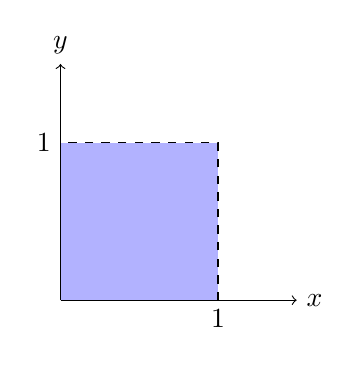
\begin{tikzpicture}
    \draw[->] (0,0) -- (3,0) node[right] {$x$};
    \draw[->] (0,0) -- (0,3) node[above] {$y$};
    \fill[blue!30] (0,0) rectangle (2,2);
    \draw[dashed] (2,0) -- (2,2) -- (0,2);
    \node[below] at (2,0) {$1$};
    \node[left] at (0,2) {$1$};  
\end{tikzpicture}
\end{center}
\begin{align*}
    &(X,Y)\sim U([0,1]^2)\\
    &f_{X,Y}(x,y)=\ind_{[0,1]^2}(x,y)=\ind_{[0,1]}(x)\ind_{[0,1]}(y)=f_X(x)f_Y(y)
\end{align*}
So $X$ is independent of $Y$
Ex2: Now consider the same distribution but for a circle instead of a square
\begin{center}
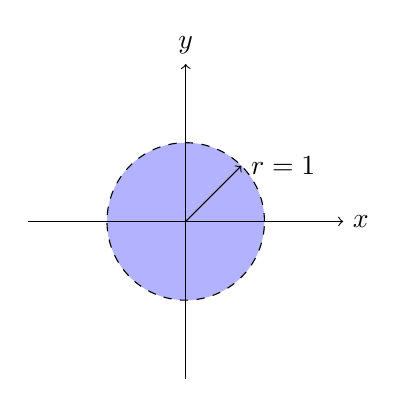
\begin{tikzpicture}
    \fill[blue!30] (0,0) circle (1);
    \draw[->] (-2,0) -- (2,0) node[right] {$x$};
    \draw[->] (0,-2) -- (0,2) node[above] {$y$};
    \draw[dashed] (0,0) circle (1);
    \draw[->] (0,0) -- (0.707,0.707) node[right] {$r=1$};
\end{tikzpicture}
\end{center}
\begin{align*}
    &(X,Y)\sim U(B_1^2(0,0))\\
    &f_{X,Y}(x,y)=\frac{1}{\pi}\ind_{B_1^2(0,0)}(x,y)=\frac{1}{\pi}\ind\brcurly{\sqrt{x^2+y^2}\leq1}\\
    &f_{X,Y}(x,y)=\frac{1}{\pi}\ind_{[-1,1]}(x)\ind\brcurly{|y|\leq\sqrt{1-x^2}}
\end{align*}
So $X$ and $Y$ are not independent\\
$X$ and $Y$ being independed implies $\expect[XY]=\expect[X]\expect[Y]$
\begin{align*}
    &\expect[XY]=\int_{-\infty}^\infty\int_{-\infty}^\infty xyf_{X,Y}(x,y)dxdy=\int_{-\infty}^\infty\int_{-\infty}^\infty xf_X(x)yf_Y(y)dxdy\\
    &=\int_{-\infty}^\infty yf_Y(y)dy\int_{-\infty}^\infty xf_X(x)dx=\expect[Y]\expect[X]
\end{align*}
So if $X$ and $Y$ are independent then $\expect[XY]=\expect[X]\expect[Y]$ however, the inverse is not always true. $\expect[XY]=\expect[X]\expect[Y]$ does not imply that $X$ and $Y$ are independent.\\
We can extend this further to functions. If $X$ and $Y$ are independent then
\[\expect[g(X)h(Y)]=\expect[g(X)]\expect[h(Y)]\]
\begin{proof}
\begin{align*}
    &\expect[g(X)h(Y)]=\int_{-\infty}^\infty\int_{-\infty}^\infty g(x)h(y) f_{X,Y}(x,y)dxdy\\
    &f_{X,Y}(x,y)=f_X(x)f_Y(y)\\
    &\expect[g(x)h(y)]=\int_{-\infty}^\infty\int_{-\infty}^\infty g(x)h(y) f_X(x)f_Y(y)dxdy=\int_{-\infty}^\infty g(x)f_X(x)dx\int_{-\infty}^\infty h(y)f_Y(y)dy\\
    &\expect[g(x)h(y)]=\expect[g(X)]\expect[h(Y)]
\end{align*}
\end{proof}
If $X$ and $Y$ are independent then we can also get a formula for the variance of $X+Y$.
\begin{align*}
    &\Var(X+Y)=\expect[(X+Y)^2]-\expect[X+Y]^2\\
    &=\expect[X^2+2XY+Y^2]-\brround{\expect[X]^2+2\expect[X]\expect[Y]+\expect[Y]^2}\\
    &=\expect[X^2]-\expect[X]^2+\expect[Y^2]-\expect[Y]^2+2\expect[XY]-2\expect[X]\expect[Y]\\
    &=\expect[X^2]-\expect[X]^2+\expect[Y^2]-\expect[Y]^2\\
    &=\Var(X)+\Var(Y)
\end{align*}
Ex: Let $X$ and $Y$ be independent random variables with known variance and expectation. What is $\expect[X^2Y]$?
\begin{align*}
    &\expect[X^2Y]=\expect[X^2]\expect[Y]\\
    &\Var(X)=\expect[X^2]-\expect[X]^2\Ra\expect[X^2]=\Var(X)+\expect[X]^2\\
    &\expect[X^2Y]=(\Var(X)+\expect[X]^2)\expect[Y]
\end{align*}

\subsection{Normal Distributions}

\subsubsection{Standardization}
Let $X$ have finite variance. Then for $Y:=\frac{X-\expect[X]}{\sqrt{\Var(X)}}$ we have $\expect[Y]=0$ and $\Var(Y)=1$.
\begin{proof}
\begin{align*}
    &\expect[Y]=\expect\brsquare{\frac{X-\expect[X]}{\sqrt{\Var{X}}}}=\frac{1}{\sqrt{\Var(X)}}\brround{\expect[X]-\expect[X]}=0\\
    &\Var(Y)=\Var\brround{\frac{X-\expect[X]}{\sqrt{\Var(X)}}}=\Var\brround{\frac{X}{\sqrt{\Var(X)}}}=\frac{1}{\Var(X)}\Var(X)=1
\end{align*}
\end{proof}
Let us now look at the example of
\[\int_{-\infty}^\infty e^{-u^2}du=\sqrt{\pi}\]
Since the exponential is non-negative, we can get that $f(u)=\frac{1}{\sqrt{\pi}}e^{-u^2}$ is a density function on $\R$. Calling a corresponding random variable $U$ we can calculate its expectation and variance as
\begin{align*}
    &\expect[U]=\int_\R u\frac{1}{\sqrt{\pi}}e^{-u^2}du=-\frac{1}{2\sqrt{\pi}}e^{-u^2}\eval_{-\infty}^\infty=0\\
    &\Var(U)=\expect[U^2]-\expect[U]^2=\expect[U^2]=\int_\R u^2\frac{1}{\sqrt{\pi}}e^{-u^2}du\\
    &=-\frac{u}{2\sqrt{\pi}}e^{-u^2}\eval_{-\infty}^\infty-\int_{-\infty}^\infty -\frac{1}{2\sqrt{\pi}}e^{-u^2}du=\frac{1}{2}\int_{-\infty}^\infty\frac{1}{\sqrt{\pi}}e^{-u^2}du=\frac{1}{2}\int_{-\infty}^\infty f_U(u)du=\frac{1}{2}
\end{align*}
This gave us a variance of $\frac{1}{2}$. We can construct a standardized version as follows:
\begin{align*}
    &X=\frac{U-\expect[U]}{\sqrt{\Var(U)}}=\frac{U}{\sqrt{\frac{1}{2}}}=\sqrt{2}U\\
    &f_X(x)=F_X'(x)\\
    &F_X(x)=\prob(X\leq x)=\prob(\sqrt{2}U\leq x)\\
    &F_X(x)=\prob\brround{U\leq\frac{x}{\sqrt{2}}}=F_U\brround{\frac{x}{\sqrt{2}}}\\
    &f_U(x)=F_U'(x)\\
    &f_X(x)=\ddx{x}F_X(x)=\ddx{x}F_U\bfrac{x}{\sqrt{2}}=F_U'\bfrac{x}{\sqrt{2}}\frac{1}{\sqrt{2}}=f_U\bfrac{x}{\sqrt{2}}\frac{1}{\sqrt{2}}\\
    &=\frac{1}{\sqrt{\pi}}e^{-\bfrac{x}{\sqrt{2}}^2}\frac{1}{\sqrt{2}}=\frac{1}{\sqrt{2\pi}}e^{-\frac{x^2}{2}}
\end{align*}
We call a random variable $X$ standard normally distributed if it has the above density. We write $X\sim\norm(0,1)$.\\
We can generalize this further to a normal distribution that has expectation (mean) $\mu$ and variance $\sigma^2$.\\
We set $Y=\sigma X+\mu$ then $\expect[Y]=\mu$ and $\Var(Y)=\sigma^2$ and we get
\begin{align*}
    &f_Y(y)=\ddx{y}F_Y(y)=\ddx{y}\prob(Y\leq y)=\ddx{y}\prob(\sigma X+\mu\leq y)=\ddx{y}\prob\brround{x\leq\frac{y-\mu}{\sigma}}\\
    &=\ddx{y}F_X\brround{\frac{y-\mu}{\sigma}}=f_X\bfrac{y-\mu}{\sigma}\frac{1}{\sigma}=\frac{1}{\sqrt{2\pi}}e^{-\frac{\bfrac{y-\mu}{\sigma}^2}{2}}\frac{1}{\sigma}=\frac{1}{\sqrt{2\pi\sigma^2}}e^{-\frac{(y-\mu)^2}{2\sigma^2}}
\end{align*}
We say that $X$ has normal or Gaussian distribution with mean $\mu$ and variance $\sigma^2$ and write $X\sim\norm(\mu,\sigma^2)$.\\
Central Limit Theorem:\\
Let $X_1,\ldots, X_n$ be independent random variables with $\expect[X_1]=\mu\in\R$ and $\Var(X_1)=\sigma^2>0$. We define $\overline{X}_n:=\frac{1}{n}\sum\limits_{i=1}^n x_i$. Then
\[\lim_{n\to\infty}\prob\brround{\frac{\overline{X}_n-\expect[\overline{X}_n]}{\sqrt{\Var(\overline{X}_n)}}\leq x}=\int_{-\infty}^x\frac{1}{\sqrt{2\pi}}e^{-\frac{u^2}{2}}\]
Other formulations of this are
\[\sqrt{n}\frac{\overline{X}_n-\mu}{\sigma}\sim\norm(0,1)\]
and
\[\frac{\sum\limits_{i=1}^n(X_i-\mu)}{\sqrt{n}\sigma}\overset{d}{\to}\norm(0,1)\]